\documentclass{TDP005mall}
\usepackage{graphicx}
\usepackage{float}


\newcommand{\version}{Version 1.2}
\author{Martin Kuiper, \url{marku849@student.liu.se}\\
  Jim Teräväinen, \url{jimte145@student.liu.se}}
\title{Designspecifikation}
\date{\today}
\rhead{Martin Kuiper\\
Jim Teräväinen}



\begin{document}
\projectpage
\section{Revisionshistorik}
\begin{table}[!h]
\begin{tabularx}{\linewidth}{|l|X|l|}
\hline
Ver. & Revisionsbeskrivning & Datum \\\hline
1.2 & Slutgiltig version med ändringar från projektets gång. Klasstrukturen har gjorts om något, och vissa ansvarsområden har flyttats mellan klasser. Fler funktioner har lagts till i klasserna. Upgrade\_Station har bytt namn till Upgrade\_Pillar. Hud ärver inte längre av Game\_Object. Spawner byttes ut mot en funktion i Game\_State. UML-diagrammet har delats upp i två delar. & 2020-12-18 \\\hline
1.1 & Ändringar i UML diagram, tick blev update på många ställen och vissa publika variabler blev private & 2020-12-03 \\\hline
1.0 & Första utkast för designspecifikationen. & 2020-11-27 \\\hline
\end{tabularx}
\end{table}

\begin{figure}[H]
         \begin{center}
             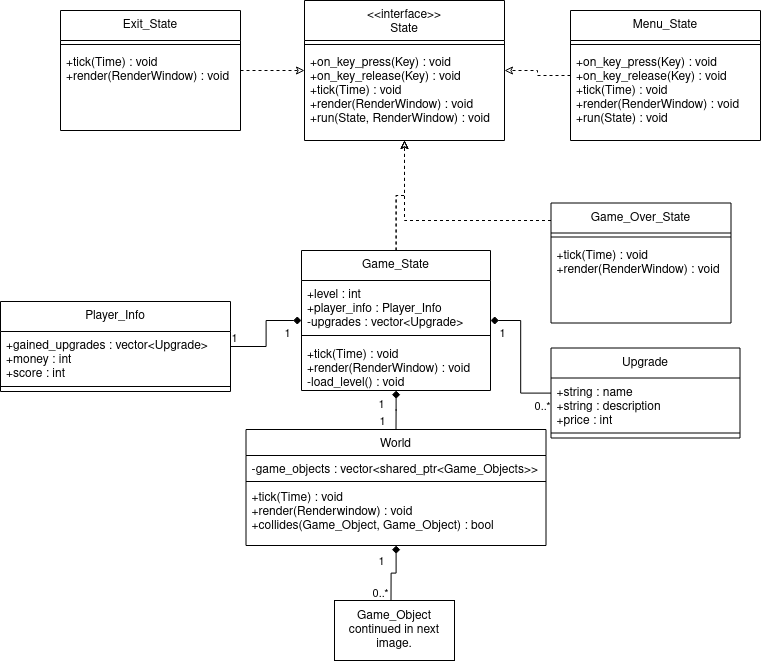
\includegraphics[width=15cm]{Graphic/overview_part1.png}
             \caption{\label{fig:1} Övergripande UML diagram för strukturen i spelet fokuserat på State och dess underklasser.}
         \end{center}
\end{figure}

\begin{figure}[H]
         \begin{center}
             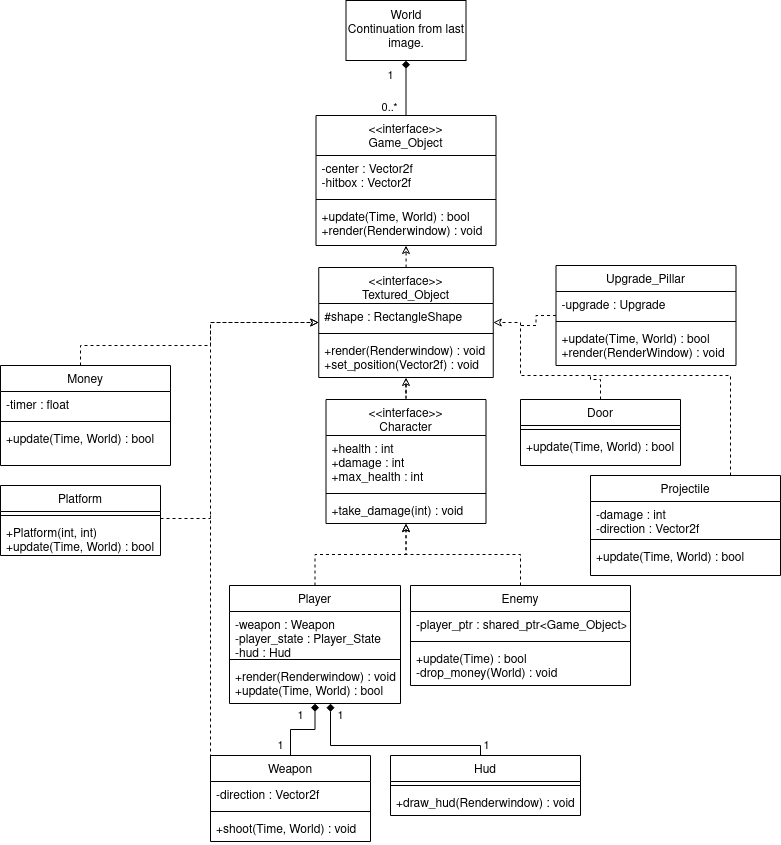
\includegraphics[width=15cm]{Graphic/overview_part2.png}
             \caption{\label{fig:1} Övergripande UML diagram för strukturen i spelet fokuserat på Game\_Object och dess underklasser.}
         \end{center}
\end{figure}
\pagebreak
\section{Beskrivning av övergripande system}

\subsection{Stadier}
Grunden för spelet ligger i att det skapas olika stadier som sedan körs och hanterar underfunktioner. Dessa stadier representeras i toppen av figur \ref{fig:1} med namn som innehåller 'state'. När spelet startar skapas ett 'Menu\_State' där spelaren kan välja mellan olika alternativ. Alternativen leder till olika saker men oftast till att spelet startas igenom att köra 'Game\_State'. 

'Game\_State' kommer att existera under hela körtiden och håller därför koll på viss information som behöver behållas. Detta inkluderar saker som hur många spelplaner spelaren klarat (level) för att skala upp svårighetsgraden. Det håller även koll på viss information som behöver vara konstant när spelaren skapas om för varje spelplan, som hur mycket pengar och vilka uppgraderingar spelaren har. Allting under 'World' kommer att försvinna och skapas igen på nya platser för varje spelplan som laddas in.

\subsection{Världen och objekt}
Världen representeras av klassen 'World' och hanterar ett obestämt antal 'Game\_Object' som alla har en position och 'hitbox'. Dessa objekt bildar tillsammans det komplexa system som är spelet. Alla objekt har en textur och ärver därmed från klassen 'Textured\_Object' som kommer hjälpa till att hantera texturerna för objekten. Klassen Game\_State har hand om att skapa och hålla koll på finderna som ska dyka upp på spelplanen. Så länge som rätt mängd fiender för nuvarande 'level' inte skapats så kommer den fortsätta att skapa fiender med ett visst tidsintervall, detta också baserat på 'level'.

Klassen 'Character' ärver från 'Textured\_Object' och innehåller allt som spelare och fiender har gemensamt, som att de har hälsa och skada. Hälsa representerar hur mycket skada en karaktär kan ta innan den raderas från spelplanen, och i spelarens fall förlorar. Hälsa är individuellt och sparas i alla objekt för sig, det går ned när objektet tar skada. Skada representerar hur mycket hälsa spelaren eller en fiende förlorar när de blir nuddade av något som gör skada.

'Player' representerar spelarkaraktären och hanterar sin rörelse, hur den reagerar på kollisioner, och sitt 'Weapon'. 'Player' kan tillkalla funktionen 'shoot()' i sitt weapon så att det avfyras en projektil i vapnets riktning. Denna projektil ärver sin skada från spelaren så att eventuella uppgraderingar som modifierar spelaren appliceras.

'Enemy' hanterar sin egen rörelse och rör sig mot spelaren för att skada denna.

\subsection{Objekt med få funktioner}
'Money' lägger till ett visst värde på spelarens pengar när de kolliderar med dem. Vi valde av tematiska skäl att visa pengarna som Själar för spelaren men funktionen är oförändrad. 

'Hud' ritar ut hur mycket hälsa och pengar spelaren har så att spelaren enkelt kan se om de är påväg att förlora eller har råd med en uppgradering. 

'Platform' hanterar de plattformar som spelaren kan stå på i nivån utöver botten av skärmen. 

'Door' skapas på kordinater enligt 'load\_level()' när alla fiender besegrats. Genom att interagera med dörren laddas nästa spelplan in. 

'Upgrade\_Pillar' skapas också enligt koordinater från 'load\_level()' när alla fiender besegrats och innehåller en slumpad uppgradering. Denna uppgradering kan läggas till i 'player\_info' om spelaren har nog med pengar (själar) för att köpa den och väljer att gör det.

\section{Klassbeskrivningar}
\subsection{Player}
Player ska kunna uppdatera sin position beroende på vilka knappar som är intryckta samt vilket state Player har.
Player har en överlagrad render()-funktion, då den behöver kunna uppdatera hur den renderas beroende på vad som händer Player-objektet.
Funktionen update() kallar alla funktioner som ska köra när spelet uppdateras. 

\subsubsection{Viktiga datamedlemmar}
\begin{itemize}
\item state - påverkar hur objektet beter sig när update() kallas.
\item weapon - ett objekt av klassen Weapon ägs av Player.
\item hud - ett objekt av klassen Hud ägs av Player.
\item activate\_popup - ett textobjekt som visas när spelaren kan interagera med vissa andra objekt.
\item player\_info - en referens till Player\_Info-objektet som håller reda på saker som spelarens insamlade score och pengar.
\item invincible - hur länge Player ska vara osårbar.
\item max\_jumps - hur många gånger Player kan hoppa utan att nudda marken.
\item health - ärvd från Character, minskar när Player tar skada.
\item damage - ärvd från Character, påverkar Players vapens skada.
\item speed - ärvd från Character, påverkar hastigheten av objektets förflyttning.
\item shape - ärvd från Textured\_Object, påverkar hur objektets textur ritas ut.
\item center - ärvd från Game\_Object, bestämmer objektets position på skärmen.
\item hitbox - ärvd från Game\_Object, bestämmer storleken på objektets kollisionsområde.
\end{itemize}

\subsubsection{Konstruktor}
Konstruktorn vi har skapat för player behöver koordinater var objektet ska starta, och en referens till Player\_Info-objektet. Resten av datamedlemmarna initieras till standardvärden.

I början av spelet får spelarkaraktären vissa startvärden på sina förmågor från funktionen apply\_upgrades. När ett nytt Player-objekt skapas på varje ny nivå tas de köpta uppgraderingarna från Player\_Info och modifierar värdena som appliceras av apply\_upgrades. 

Player-konstruktorn kallar i sin tur Textured\_Object-konstruktorn, vilken Player ärver. Den sätter players hitbox automatiskt till samma storlek som texturen. Det är väldigt smidigt i de flesta fall, men då vi vill att Player ska vara animerad och av effektivitetsskäl använda samma textur för alla animationsbilder blir Players hitbox mycket större än önskat. Därför justeras den i Players konstruktor. 

Hitboxen justeras även för hattens bredd, då den sticker utanför resten av kroppen.

Funktionen setup\_activate\_popup() kallas för att ställa in textrutan som ska visas när Player-objektet står framför ett objekt spelaren kan interagera med. 

\subsubsection{update(Time)}
Vid varje uppdatering av spelet kallas Players update-funktion av det ägande World-objektet. Funktionen har i uppdrag att utföra följande:

För att flytta Player kallas move\_player().

För att flytta och skjuta vapnet kallas handle\_weapon().

För att hantera Players kollisionsbeteende med andra objekt kallas handle\_collision().

För att hantera animationerna av Players textur kallas handle\_animation().

Datamedlemmen 'invincible' minskas med tiden som passerat sen den senaste uppdateringen om den inte är 0.

Det ägda Hud-objektets datamedlemmar uppdateras så att nuvarande hälsa, pengar och poäng visas på skärmen. 

En datamedlem i Player\_Info uppdateras så att Game\_State vet om spelaren har dött eller inte.

Slutligen returneras spelarens levandestatus till World så att den inte tas bort om den inte är död.

\subsubsection{move\_player()}
För att hantera den horisontella rörelsen kallas funktionen handle\_horizontal\_move().
Den flyttar karaktären beroende på vilka tangenter som är intryckta.

För att hantera hopp-input kallas handle\_jump\_input().
Den ser till att när spelaren trycker på hopp-knappen ändras state till 'jumping' om spelaren inte redan hoppat maximalt antal gånger utan att landa. 

För att kolla om spelaren ska börja falla från en platform kallas funktionen handle\_drop().

Om player\_state är satt till 'jumping' kallas jump() för att hantera hopp-rörelsen.
Efter en viss tid sätter jump() player\_state till 'falling'.

Om player\_state är satt till 'falling' kallas fall() för att hantera fall-rörelsen.

Normalt är player\_state satt till 'standing'. 


\subsubsection{handle\_weapon()}
Players position bestämmer Weapon-objektets position. 

Input från tangentbord eller muspekare bestämmer vapnets rotation.
Vapnet har en datamedlem 'fire\_rate' som påverkar hur ofta det kan avfyras. 

Är 'Avfyra vapen'-knappen intryckt och vapnets 'fire\_rate' 0 skapas en projektil.
Projektilen rör sig i riktningen av vapnets rotation och har en datamedlem 'damage' som sätts till Players 'damage'.

\subsubsection{handle\_collision(World)}
Player frågar World vilka objekt den kolliderar med. 

Om den understa delen av Player-objektet kolliderar med den översta delen av en plattform och player\_state är 'falling' ändras player\_state till 'standing'.

Kolliderar Player med ett Enemy-objekt och 'invincible' är noll kallas take\_damage(). Spelaren får även audiovisuell respons på att den tagit skada och 'invincible' ökas med odödlighetsperioden.

Kolliderar Player med ett Upgrade\_Pillar- eller  Door-objekt visas hjälptexten i 'activate\_popup'.

Om 'Bekräfta val'-knappen är intryckt köper spelaren uppgraderingen på Upgrade\_Pillar om den har råd och uppgraderingen inte redan är köpt. 

Om 'Bekräfta val'-knappen är intryckt vid kollision med 'Door'-objekt signalerar Player via Player\_Info till Game\_State att nästa nivå ska laddas in.

\subsubsection{handle\_animation()}
Spelarens textur uppdateras baserat på om spelaren aktivt rör sig i x-led eller inte, och vilken riktning den har. Vid rörelse spelas en animationsslinga upp baserat på nuvarande x-position.

\subsection{World}
World har i uppdrag att hantera alla spelets Game\_Object-objekt. World ägs av Game\_State, som även kallar vissa av Worlds publika funktioner varje gång spelet ska uppdateras och renderas.  

\subsubsection{Datamedlemmar}
\begin{itemize}
\item game\_objects  - Vector som innehåller smartpekare till alla Game\_Object-objekt.
\item stored\_window - Referens till objektet som hanterar spelfönstret (RenderWindow). Behövs för att hålla rätt på var muspekaren är relativt till fönstret.
\end{itemize}

\subsubsection{Konstruktor}
Worlds konstruktor tar in en referens till programfönsterobjektet av klass RenderWindow. Default-konstruktorn är avstängd då stored\_window alltid måste initialiseras till rätt värde för att spelet ska fungera. 

\subsubsection{tick(Time)}
Funktionen kallas mellan varje rendering av Game\_State, som skickar med tidsskillnaden sedan förra gången funktionen kallats. 

Worlds lista av Game\_Object-smartpekare loopas igenom och den virtuella funktionen update() kallas i varje objekt. Barnklasserna av Game\_Object överlagrar update() och utför de unika handlingar som passar den typen av objekt. 

En referens till World-objektet skickas med som parameter i update() för att spelobjekten ska ha tillgång till Worlds medlemsfunktioner.

De får även med tidsskilnaden delta så att de kan justera sitt beteende efter tid, vilket behövs för att förhindra att simuleringen går snabbare eller långsammare beroende på hur snabbt datorn kör koden. 

Om World får false i retur av objektets update() vet den att objektet vill raderas. Efter att ha raderat ett objekt minskar word antal gånger loopen ska köras för att unvika segmenteringsfel.

\subsubsection{render(RenderWindow)}
World loopar efter uppdateringen av alla objekt igenom objekten igen och kallar på deras renderingsfunktion, som är överlagrad på samma sätt som update(). 

En referens till programfönsterobjektet RenderWindow från SFML-biblioteket skickas till spelobjektet för att det ska kunna rita sig själv på skärmen med hjälp av RenderWindows medlemsfunktioner.

\subsubsection{clear\_level()}
Mellan varje nivå rensas worlds spelobjektslista helt med clear\_level() så att nya objekt kan laddas in.

\subsubsection{add\_front(), add\_back() och insert\_at()}
För att lägga till nya spelobjekt, exempelvis projektiler, kallas någon av tilläggningsfunktionerna. 

Då vissa saker ska renderas framför andra saker, som spelarkaraktären framför platformarna, så har vi olika funktioner för att lägga till saker först eller sist i listan.

I ett fall vill vi att uppgraderingspelarna ska läggas framför platformar men bakom allt annat, då kallas funktionen insert\_at() av Game\_State som själv håller reda på hur många platformar som skapats. 

\subsubsection{collides() och collides\_with()}
När ett spelobjekt vill veta om det kolliderar med några andra objekt kallar de funktionen collides\_with() och skickar med en referens till sig själva som parameter. 

World loopar igenom alla sina spelobjekt och kontrollerar med collides()-funktionen om något objekts hitbox överlappar med det första objektets hitbox. Smartpekare till alla objekt som gör detta läggs till en lista som returneras till spelobjektet.

\section{Designens för- och nackdelar}
Målet är att hålla designen så simpel som möjligt genom att designa klasser som ärver så mycket funktion som möjligt. I vissa fall kan detta spara mycket jobb då klasserna inte kräver så lång kod. Nackdelen med detta är att designen har mycket beroende av föräldrar i alla klasser och det kan vara svårt att skapa mer nischat beteende.

Då spelet har många komponenter och subsystem som interagerar med varandra kan det lätt bli väldigt komplext och oöverblickbart. För att motverka detta krävs god organisation och bra abstraktionsnivåer. 

Om det hade funnits många fler objekt med animationer hade det antagligen varit värt att lägga ut den specialkod som behövs till en separat klass mellan Textured\_Object och Character som kunnat heta Animated\_Object. Nu bedöms det inte som värt tiden att göra den refaktoreringen. 

Systemen för att skapa uppgraderingar och bandesigner har vissa för- och nackdelar som diskuteras i nästa sektion. 

En nackdel de båda delar är att det inte finns någon felhantering av filinläsningen, vilket ställer högre krav på användaren att formatera filerna korrekt.

\section{Externa filformat} 
\subsection{Bandesign}
Funktionen 'load\_level()' i 'Game\_State' använder textfiler med definerade nivåer. Funktionen läser tecken enligt en fördefinerad struktur för placering av plattformar, spelare, uppgraderingsstationer och avslutningsdörr. 

Med detta så kan man enkelt skapa nya nivåer. Detta system har även fördelen att man inte riskerar placera flera saker på samma plats då textfiler inte godkänner flera tecken på varandra.

Nackdelen är att friheten i bandesignen begränsas något.

\subsection{Uppgraderingar}
Uppgraderingarna läses också in från en textfil enligt en bestämd struktur. Det går enkelt att ändra på pris och hur mycket uppgraderingen ska ändra på spelarkaraktärens förmågor. 

Det krävs en något större arbetsinsats med förändringar i koden för att lägga till uppgraderingar som ändrar annan spelardata än de kategorier som redan är implementerade. 

Exempelvis, om en uppgradering ska ändra på hur länge en spelare är odödlig efter att ha tagit skada måste förändringar göras i både load\_upgrades() i Game\_State och apply\_upgrades() i Player. Det krävs dock inte stora förändringar i någon av funktionerna och det skulle gå relativt snabbt att implementera. 

\end{document}
